\chapter{序論}
\section{研究の背景と目的}
%1章では現在youtubeなどのサービスが盛んでありそこで問題になっている動画内の楽曲とその著作権云々カンヌンを書く。著作権
%商用利用、何が問題なのか、AIならどうしていけるか、どこまでできるのか、その利用方法とこれから
\subsection{動画共有サイトの発展}
スマートフォンの発展とともに2016年の日本のインターネット利用者数は1億84万人,人口普及率は83.5%となった(総務省2017)。インターネット上の映像を容易に再生可能なスマートフォンやタブレットなどのデバイスが普及したことで,DVD等と同等の高品質な映像を視聴,配信可能なYoutube\cite{webpage}やニコニコ動画\cite{webpage9}などの動画共有サービスの発展も著しく,
コンテンツデリバリーサービス(Contents Delivery Service:CDS)や各種クラウドサービスの発展により,提供側のサーバなどの構築に必要な費用が非常に低くなる中で,インターネット上に多様な映像配信サービスが提供されている。誰でも利用でき,非常に幅広いコンテンツが投稿,視聴されているが,近年,動画内に使用されている楽曲などの著作権を侵害する動画が投稿されるケースが多く社会問題になっている.
\subsection{音楽と著作権}
著作権法では,著作物を「思想又は感情を」「創作物に」「表現したもの」で,「文芸、学術、美術又は音楽の範囲に属するもの」と定義している.音楽の著作物には,曲のほかに歌詞も含まれ,録音や記譜されている必要はなく,即興演奏のような形で表現されたものも著作物である.(著作権法2条1項1号)
また著作権は,演奏権,複製権(コピー),公衆送信権(インターネットでの配信)など,利用方法ごとに「○○権」と権利が定められており,それぞれの権利に対して利用の都度、著作者の許諾が必要となっている.(著作権法21条~28条)つまり,動画共有サイト内で動画を配信する際にBGM等で著作物等を使用している場合にはその都度,権利者から許諾を得てから利用しなければならない.
\newpage
\subsection{AIによる作品と著作権}
著作権法では前項であげたように定義している.しかし現時点のAIでは「思想又は感情を」持っているとは認められず,自らの「思想」「感情」に基づいて作品を作っているわけではない.よってAIの作品に著作権は認められず,その音楽は「誰のものでもない」ということになる.これには諸説あるが具体的に法整備が行われておらず,現在ではこれが一般的な考え方である.
また,AIの学習の際に用いた解析用データに関しては,電子計算機による情報解析目的のための著作物利用が認められている.(著作権法47条7項)
よって,AIによる楽曲制作で有用な結果が得られれば,動画共有サイト等で利用する場合に自由に利用できるため,このような社会的問題を解決するために非常に有効であると言える.
\subsection{AI楽曲作成サービス}
現在,AIを用いた楽曲作成サービスはJukedeck\cite{webpage10}やAmper Music\ref{fig:Amper Music}\cite{webpage11}など様々なものが出回っている.例えばAmper Musicでは「作成したい音楽ジャンル」と「曲の長さ」を指定すれば,AIがオリジナル曲を作曲してくれるという非常に高度なサービスであるある. 
作成した曲は,テンポを変えたり,楽器を追加したりと後からも編集できるようにもなっている.このようなサービスでは個人的であれば著作権フリーで利用できるが,商用利用に関してはサービスごとに利用規約で定められており,利用できるものとそうでないものがある.\\
\begin{figure}[!ht]
    \begin{screen}
    \begin{center}
        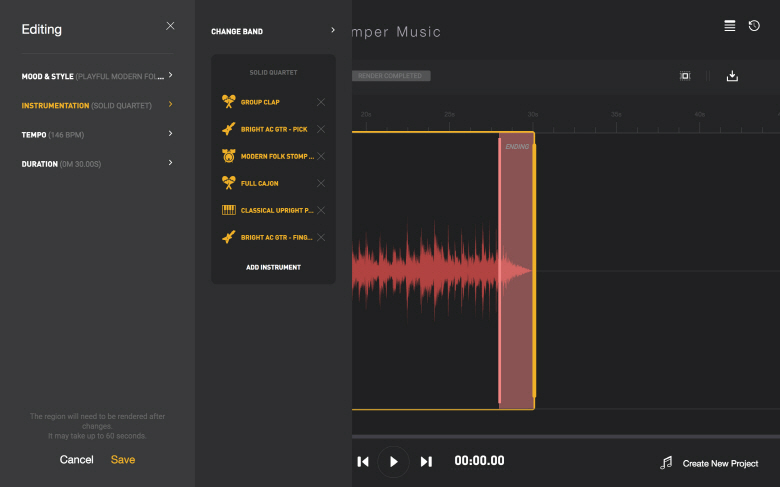
\includegraphics[scale=0.8, clip]{./img/Amper1.jpg}
        \caption{Amper Musick}
        \label{fig:Amper Music}
    \end{center}
\end{screen}
\end{figure}
\newpage
\subsection{研究の目的}
こうした背景をもとに,本研究ではAIによる楽曲生成についてGoogole brainによって公開されているTensorflowのライブラリであるMagentaを用いて実証実験を行う.これによってAIによる楽曲制作は有用なものなのか,どのような条件で楽曲を生成すれば良い結果を得られるかを調査することが目的である.\\
 実際に人間の手で楽曲を制作する際は音楽理論をもとにコードやスケールに注意して制作をする.また,どの音を使えば気持ちが良いかなど人間の感情的な部分も制作を左右する.しかしAIに感情はなく,気持ちが良い,悪いなどの判断をすることは不可能である.
そこでMagentaを用いてAIの楽曲制作ではどこまでの楽曲を制作できるのか,学習データやノード数による楽曲の生成結果の違いを比較,検証し,これが有用なものか調査する.\\
\newpage
\section{本論文の構成}
本論文の構成は以下の通りである.\\
第1章では本論文の背景と目的について述べている.\\
第2章では本論文で利用する理論について述べている.\\
第3章では実験内容について述べている.\\
第4章では楽曲制作について述べている.\\
第5章ではAIを用いた楽曲制作についての本研究の結論について述べている.\\